\chapter{実証}\label{chapter:Demonstration}
\cref{chapter:Demonstration}では, \cref{chapter:Definition}で定義したパズルルールがよく定義できているか確認を行う. \cref{section:ExistsPuzzleRule}では既存のパズルルールのうち\cref{chapter:Definition}で定義したパズルルールとして説明できるものがあることを実証する. さらに\cref{section:NewPuzzleRule}ではパズルルールの自動作成の足掛けとして新しいパズルルールが作成できることを説明する.

\section{既存のパズルルール}\label{section:ExistsPuzzleRule}
今節では既存のパズルルールが\cref{chapter:Definition}で定義したパズルルールで記述できることを実証する. \textit{codomain}, HI, \textit{identification}は自明であるから\textit{conditions}と本来のパズルルールとの対応についてのみ説明を行い, 厳密な証明は省く.
実証例としてスリザーリンクとナンバーリンクを用いる. スリザーリンクのパズルルールは\cref{example:SlitherLinkRule}である. ナンバーリンクのパズルルールは以下のものである(\cite{web:NumberLink}).
\begin{example}[ナンバーリンクのパズルルール]\label{example:NumberLinkRule}\textup{}
  \begin{enumerate}
    \item \jaitalic{白マスに線を引いて, 同じ数字どうしをつなげましょう.}\label{NumberLinkRule_1}
    \item \jaitalic{線は, マスの中央を通るようにタテヨコに引きます. 線を交差させたり, 枝分かれさせたりし}\\\jaitalic{てはいけません.}\label{NumberLinkRule_2}
    \item \jaitalic{数字の入っているマスを通過するように線を引いてはいけません.}\label{NumberLinkRule_3}
    \item \jaitalic{1マスに2本以上の線を引いてはいけません.}\\(文章は \cite{web:NumberLink}から引用. )\label{NumberLinkRule_4}
  \end{enumerate}
\end{example}

\begin{example}[スリザーリンクの数学的記述]
  スリザーリンクの\textit{codomain}, \textit{conditions}, HI, \textit{identification}はそれぞれ\cref{example:SlitherLinkCodomain}, \cref{example:SlitherLinkConditions}, \cref{example:SlitherLinkHiddenInformation}, \cref{example:SlitherLinkIndentification}である. \textit{conditions}に関し, \cref{example:SlitherLinkRule}の\ref{SlitherLinkRule_1}と\ref{SlitherLinkRule_3}は\cref{equation:SlitherLinkConditions_2}と\cref{equation:SlitherLinkConditions_3}に対応する. \cref{example:SlitherLinkRule}の\ref{SlitherLinkRule_2}は\cref{equation:SlitherLinkConditions_1}に対応している.

  このパズルルールから具体的に完成盤面を選んだものに\cref{figure:SlitherLink}の下図が含まれる. 非完成盤面は\cref{figure:SlitherLink}の上図であり, 確かにこれはスリザーリンクの(\cref{figure:SlitherLink}の完成盤面に対応する)問題の元であることが分かる.
\end{example}

\begin{example}[ナンバーリンクの数学的記述]
  ナンバーリンクは, 以下に示す\textit{codomain}, \textit{conditions}で定めた盤面をリプレイスすることによりナンバーリンクの盤面を表すことができる.
  \textit{codomain}は以下のように記述することができる
  \begin{align}
     & \mathbb{P}=\emptyset                                             \\
     & \mathbb{C}=\{\,\textit{null}, \emptyset ,x_1,x_2,\ldots, x_a\,\} \\
     & \mathbb{E}=\{\,\textit{null},0,1\,\}          .                  \\
  \end{align}

  \textit{conditions}は以下のように記述することができる
  \begin{align}
     & B\ni \forall p(i,j),1\le \textit{cross}(p(i,j))\le 2                          \label{equation:NumberLinkConditions_1} \\
     & B\ni \forall p(i,j), \textit{cross}(p(i,j))= 2 \Rightarrow p_{i,j}=\emptyset \label{equation:NumberLinkConditions_2}  \\
     & \forall G_z\ni P_z, |\{\,p(i,j)\mid cross(p(i,j))=1\,\}|=2             \label{equation:NumberLinkConditions_3}        \\
     & \forall G_z\ni P_z, \textit{cross}(p(i,j))= 1 \Rightarrow p_{i,j}=x_a     \label{equation:NumberLinkConditions_4} .   \\
  \end{align}

  HIは以下のように記述することができる
  \begin{equation}
    \{\,e_{i,j}\,\}.
  \end{equation}

  \textit{identification}は以下のように記述することができる
  \begin{equation}
    e:\textit{null}\leftrightarrow 0.
  \end{equation}

  \textit{conditions}に関し, それぞれ\cref{example:NumberLinkRule}の\ref{NumberLinkRule_1}は\cref{equation:NumberLinkConditions_1}と\cref{equation:NumberLinkConditions_2}と\cref{equation:NumberLinkConditions_4}に含まれる. \ref{NumberLinkRule_2}は\cref{equation:NumberLinkConditions_3}に対応する. \ref{NumberLinkRule_2}は\cref{equation:NumberLinkConditions_4}に含まれる. \cref{example:NumberLinkRule}の\ref{NumberLinkRule_4}は\textit{codomain}の時点で保証される.

  このパズルルールから具体的に完成盤面を選んだものは\cref{figure:NumberLink}であり, 非完成盤面は\cref{figure:NumberLinkQuestion}である. これらをリプレイスしたものがそれぞれ\cref{figure:NumberLinkReplace}, \cref{figure:NumberLinkQuestionReplace}である. これは確かにスリザーリンクの完成盤面であることが分かる.
\end{example}

\section{新しいパズルルールの作成}\label{section:NewPuzzleRule}
\cref{section:NewPuzzleRule}では\cref{chapter:Definition}において定義したパズルルールで, 新しいパズルルールが作成できることを説明する. まず, 以下のように\textit{codomain}, \textit{conditions}, HI, \textit{identification}を次のように選ぶ.

\textit{codomain}は以下とする
\begin{align}
   & \mathbb{P}=\emptyset                       \\
   & \mathbb{C}=\{\,\textit{null},0,1,2,3,4\,\} \\
   & \mathbb{E}=\{\,\textit{null},0,1\,\}  .    \\
\end{align}
\textit{conditions}は以下とする
\begin{align}
  A\ni \forall G_z, G_z\ni L_z, |L_z|=4 \\
  B\ni \forall c(i,j), c_{i,j}= cycle(c(i,j)).
\end{align}
HIは以下とする
\begin{align}
  \{\,e(i_y,j_y,y)\,\}.
\end{align}
\textit{identification}は以下とする
\begin{align}
  e:\textit{null}\leftrightarrow 0.
\end{align}

\textit{codomain}, \textit{conditions}, HI, \textit{identification}を選んだとき, 非完成盤面と完成盤面の組み合わせとして\cref{figure:NewPuzzleRule}を考えることができる(非完成盤面であることの証明は省く).

この新しく作成したパズルルールは, 以下のように定性的に記述することができる. ただし, 以下の記述は本研究を知らなくても理解できるように, 本研究で用いた線とは違う意味で用いていることに注意する.

\begin{enumerate}
  \item 長さが4のひとつながりの線を書くこと.
  \item 各マス(細胞)の数字は周りにある辺の本数である. 例えば, 2が入っているマスの周りには2本しか辺がない.
\end{enumerate}

\begin{clearpagefigure}
  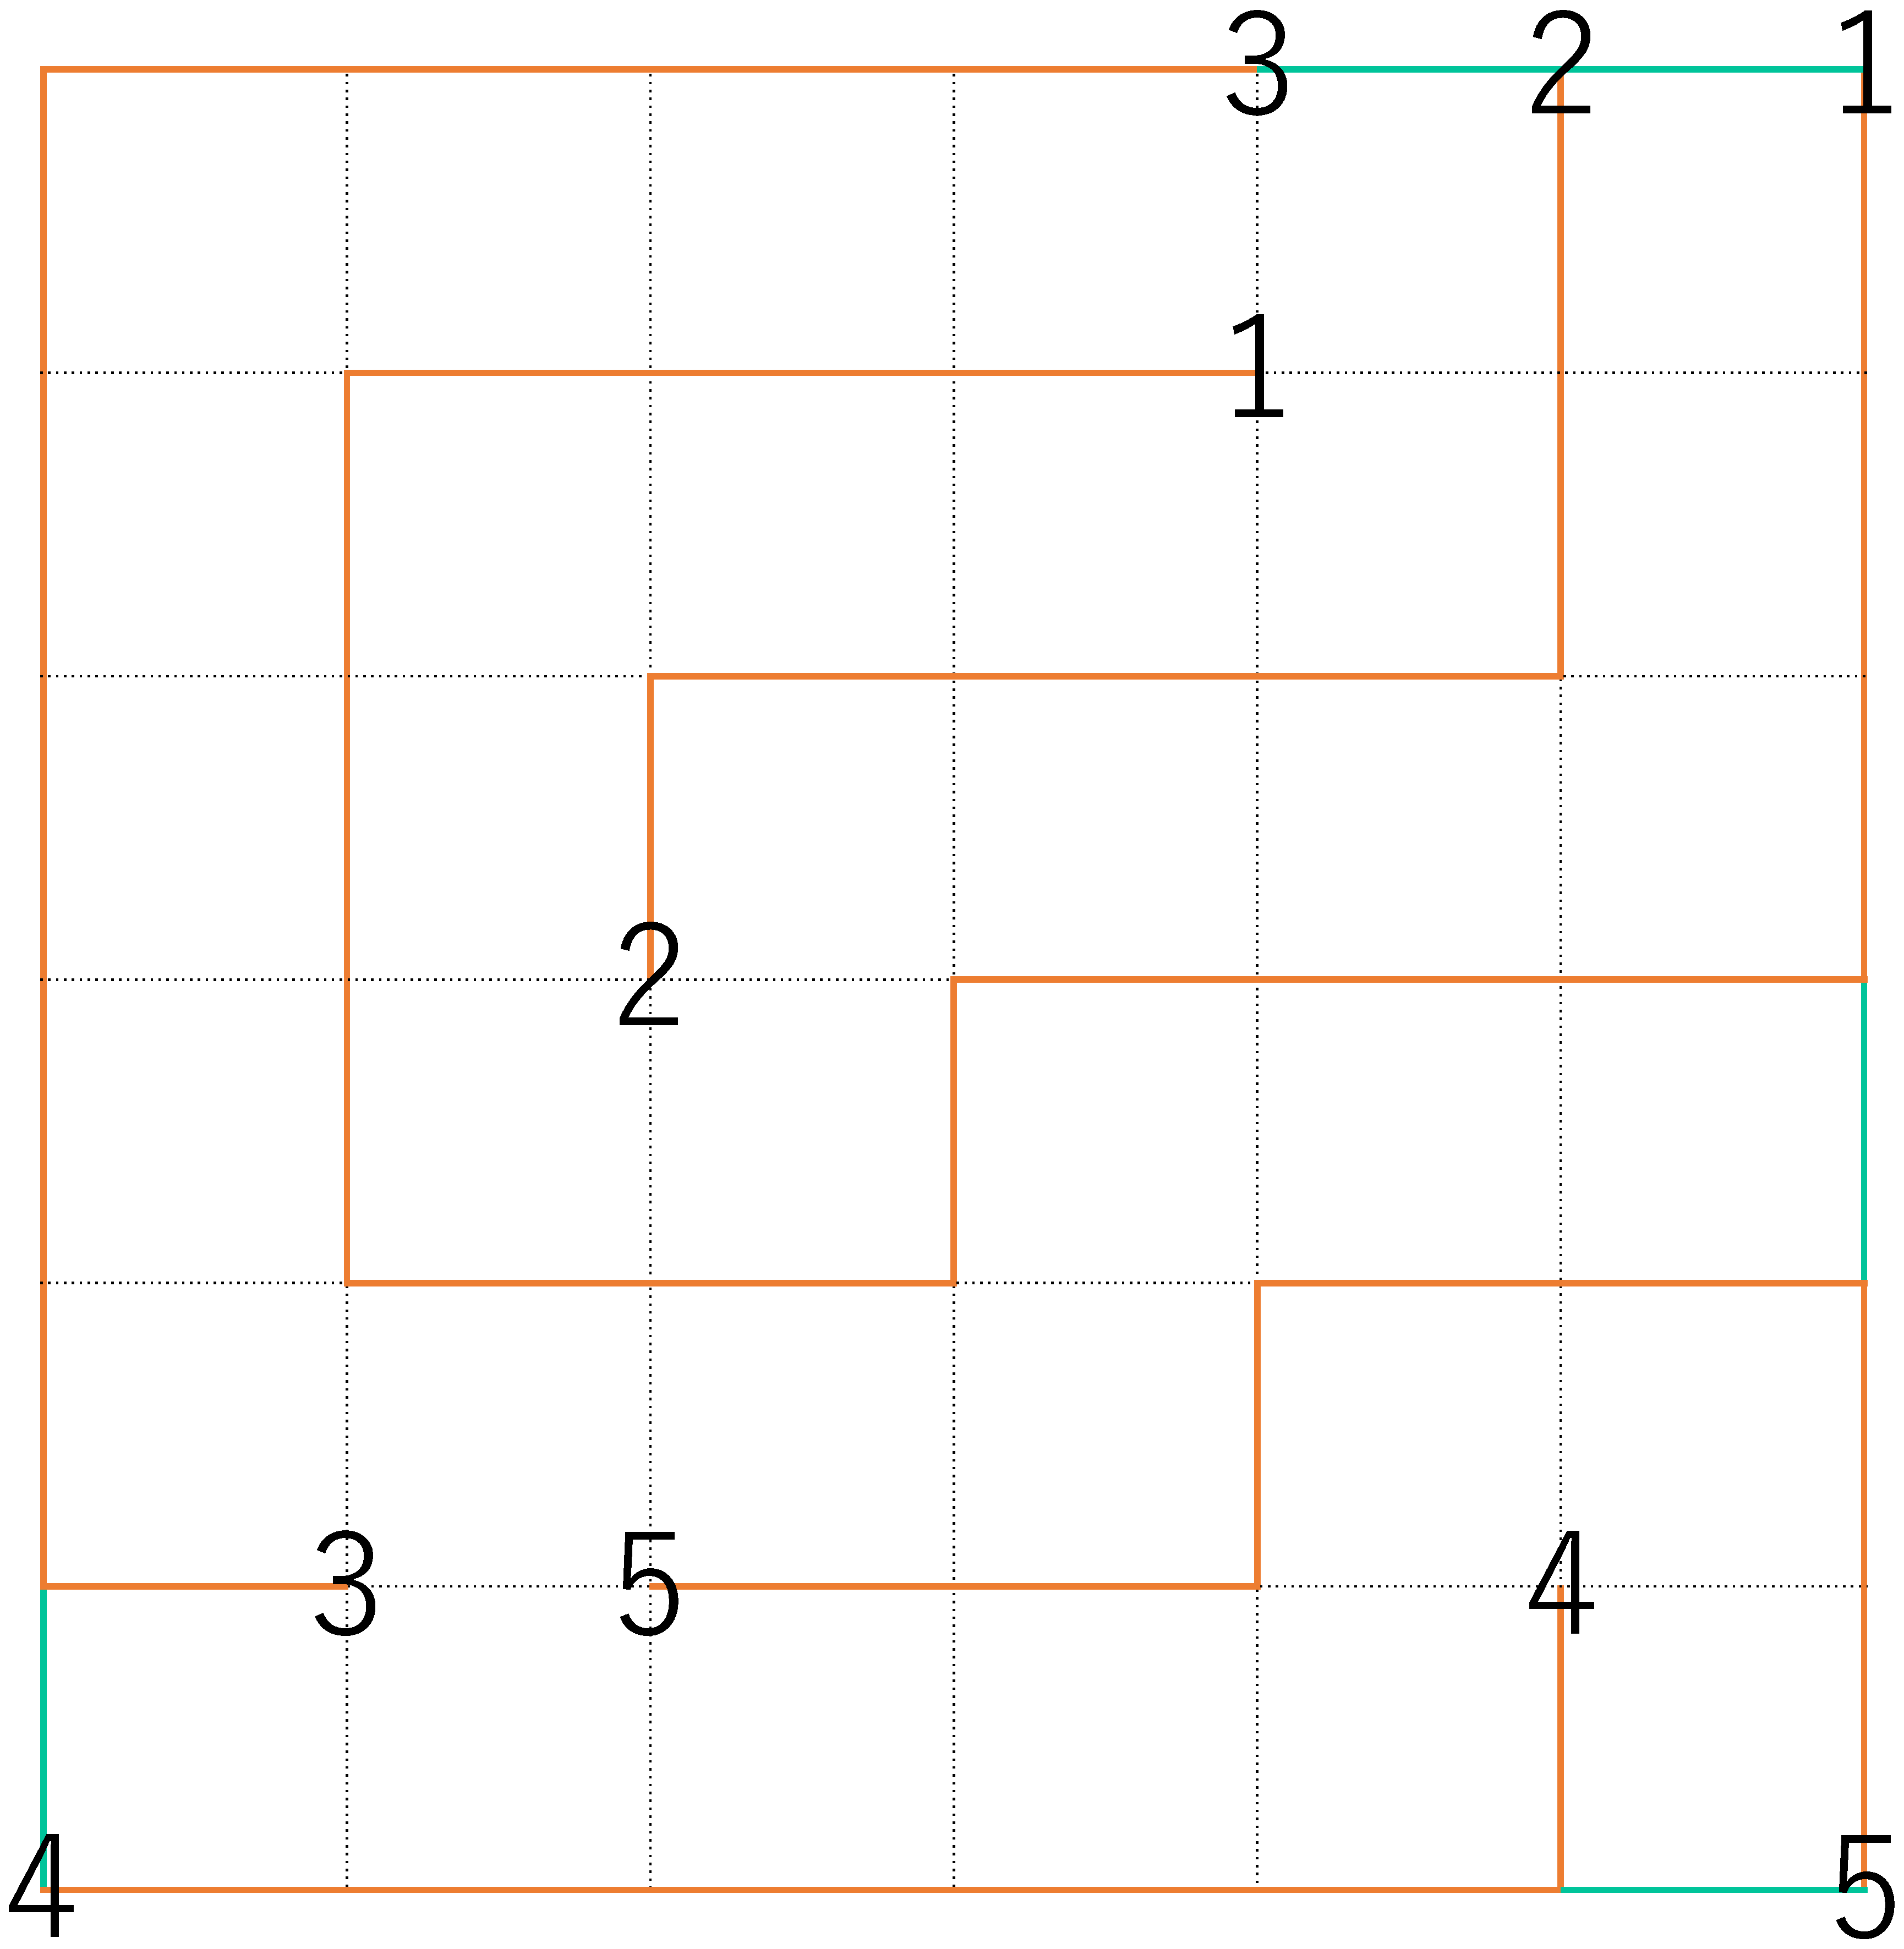
\includegraphics[width=0.85\linewidth,clip]{fig/NumberLink.eps}
  \caption{ナンバーリンクの完成盤面(リプレイス前)}
  \label{figure:NumberLink}
\end{clearpagefigure}

\begin{clearpagefigure}
  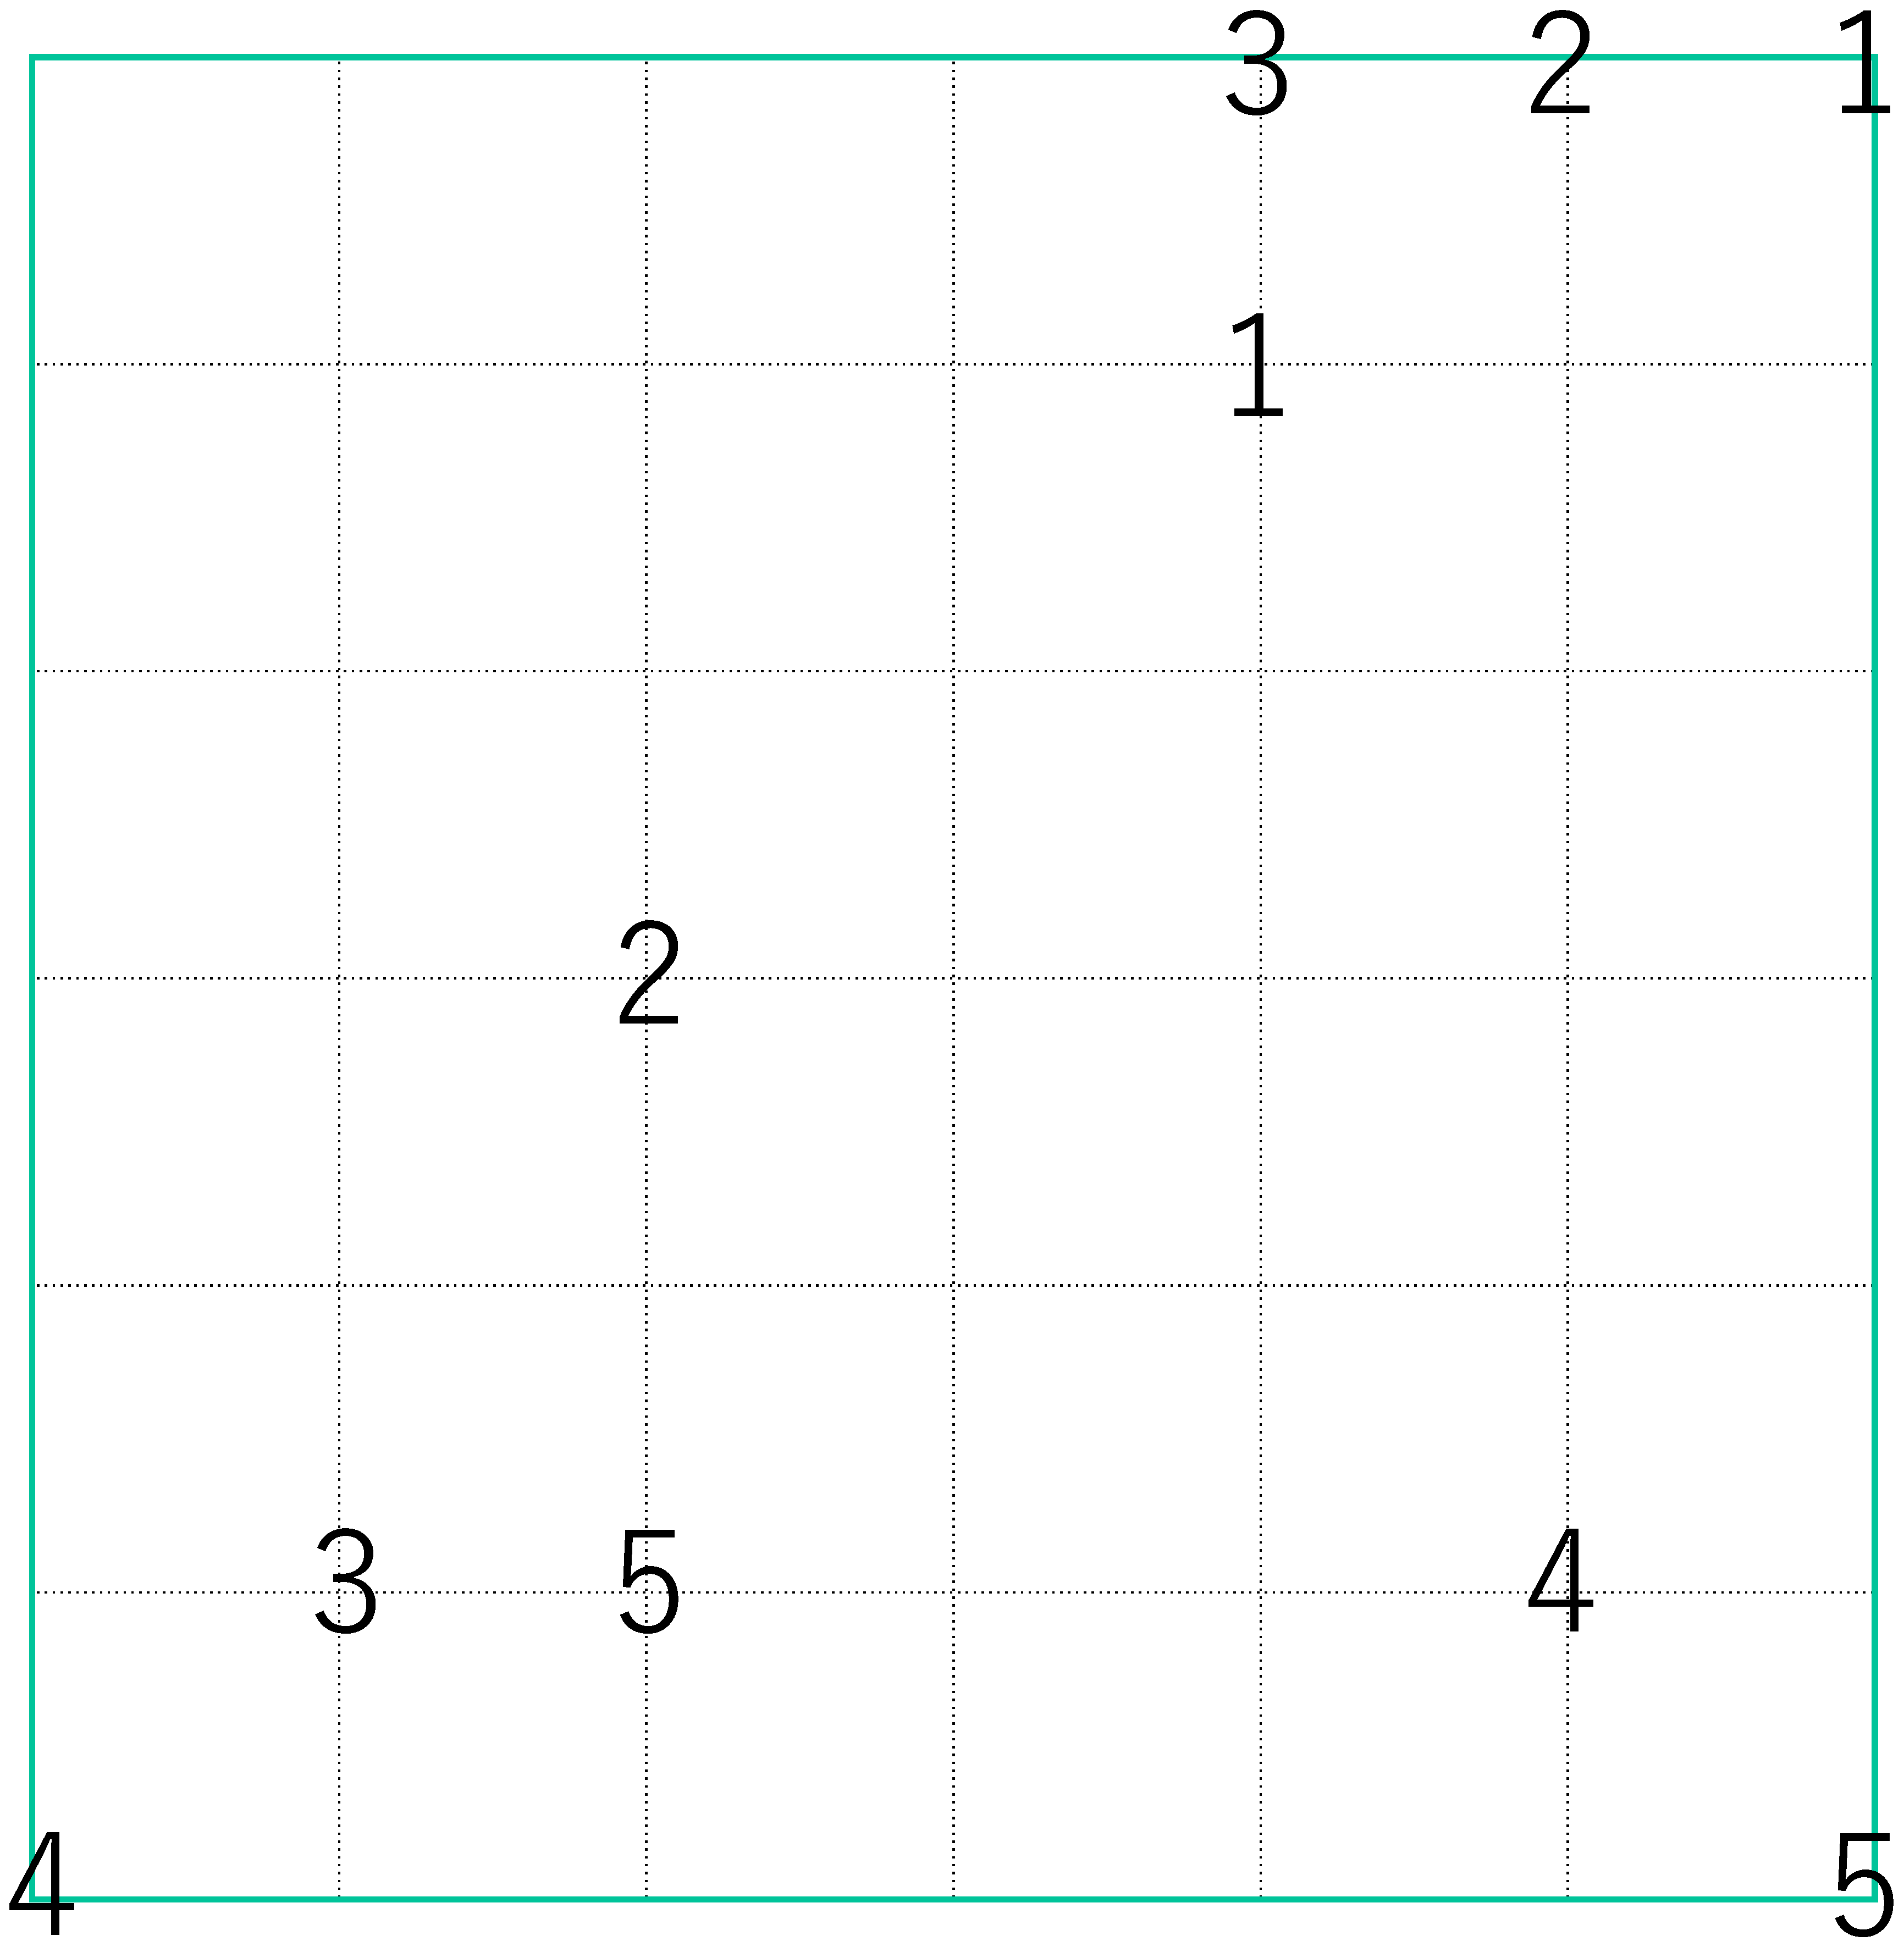
\includegraphics[width=0.85\linewidth,clip]{fig/NumberLinkQuestion.eps}
  \caption{ナンバーリンクの非完成盤面(リプレイス前)}
  \label{figure:NumberLinkQuestion}
\end{clearpagefigure}

\begin{clearpagefigure}
  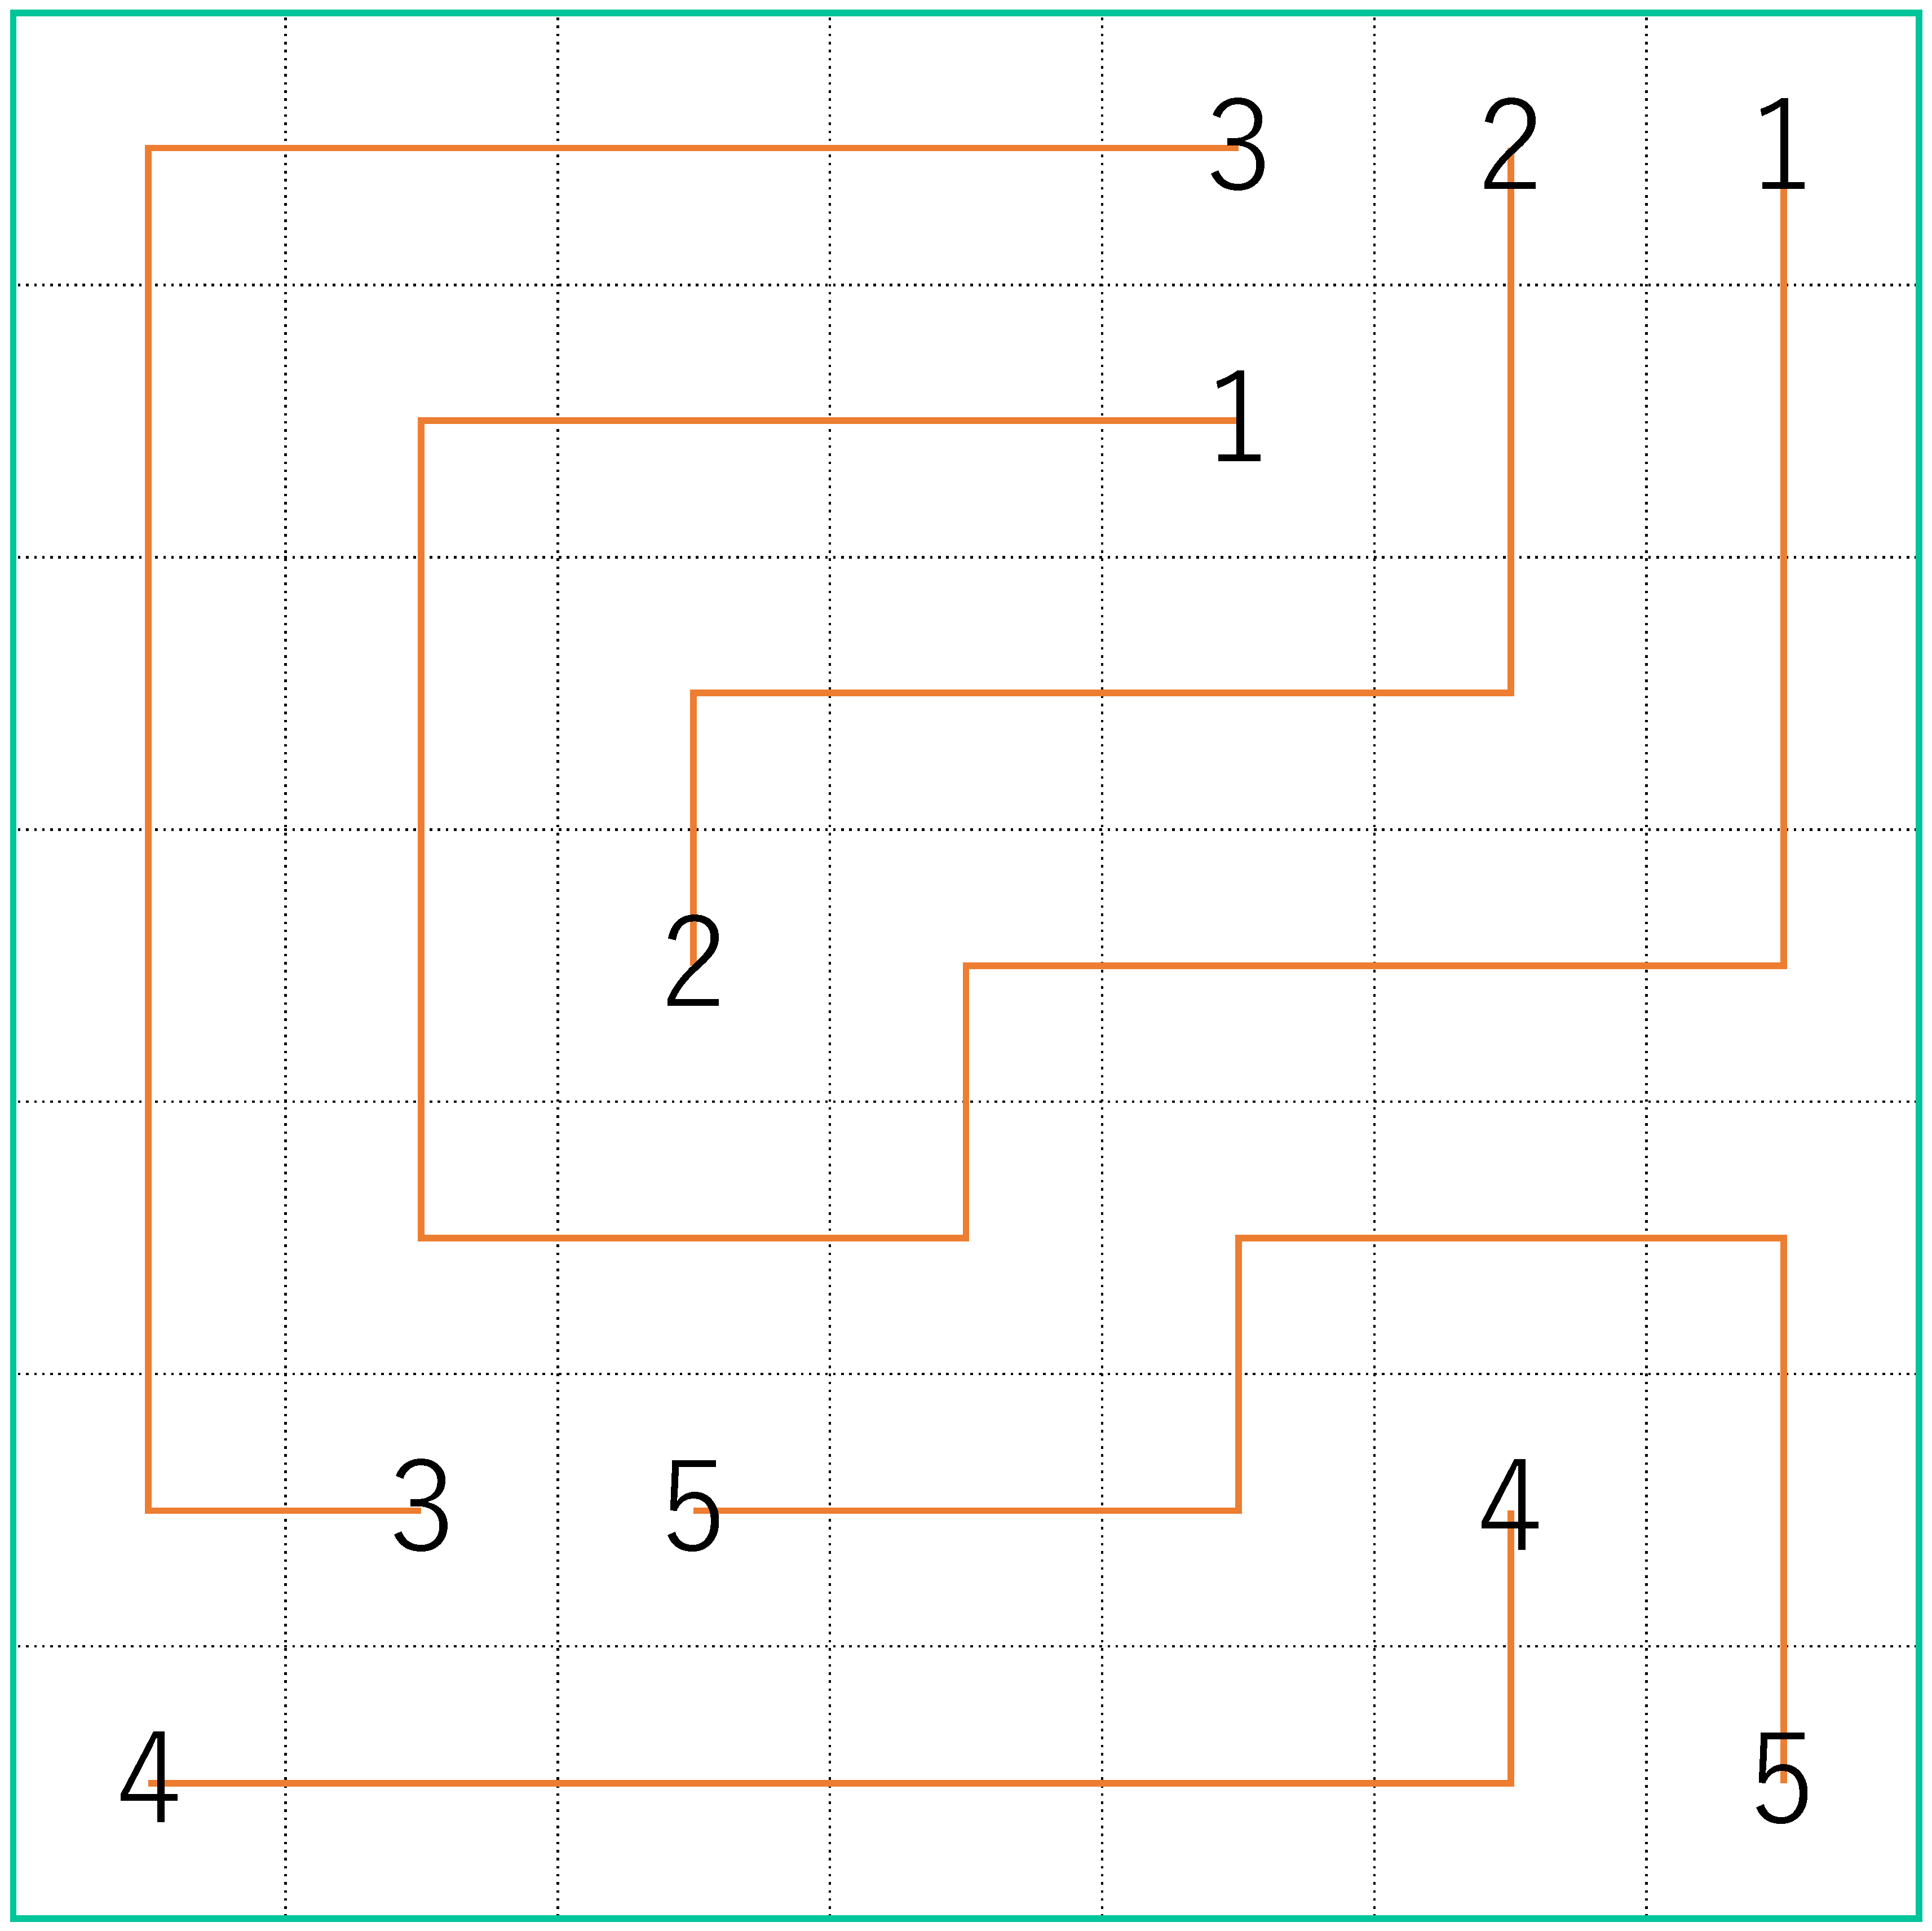
\includegraphics[width=0.85\linewidth,clip]{fig/NumberLinkReplace.eps}
  \caption{ナンバーリンクの完成盤面(リプレイス後)}
  \label{figure:NumberLinkReplace}
\end{clearpagefigure}

\begin{clearpagefigure}
  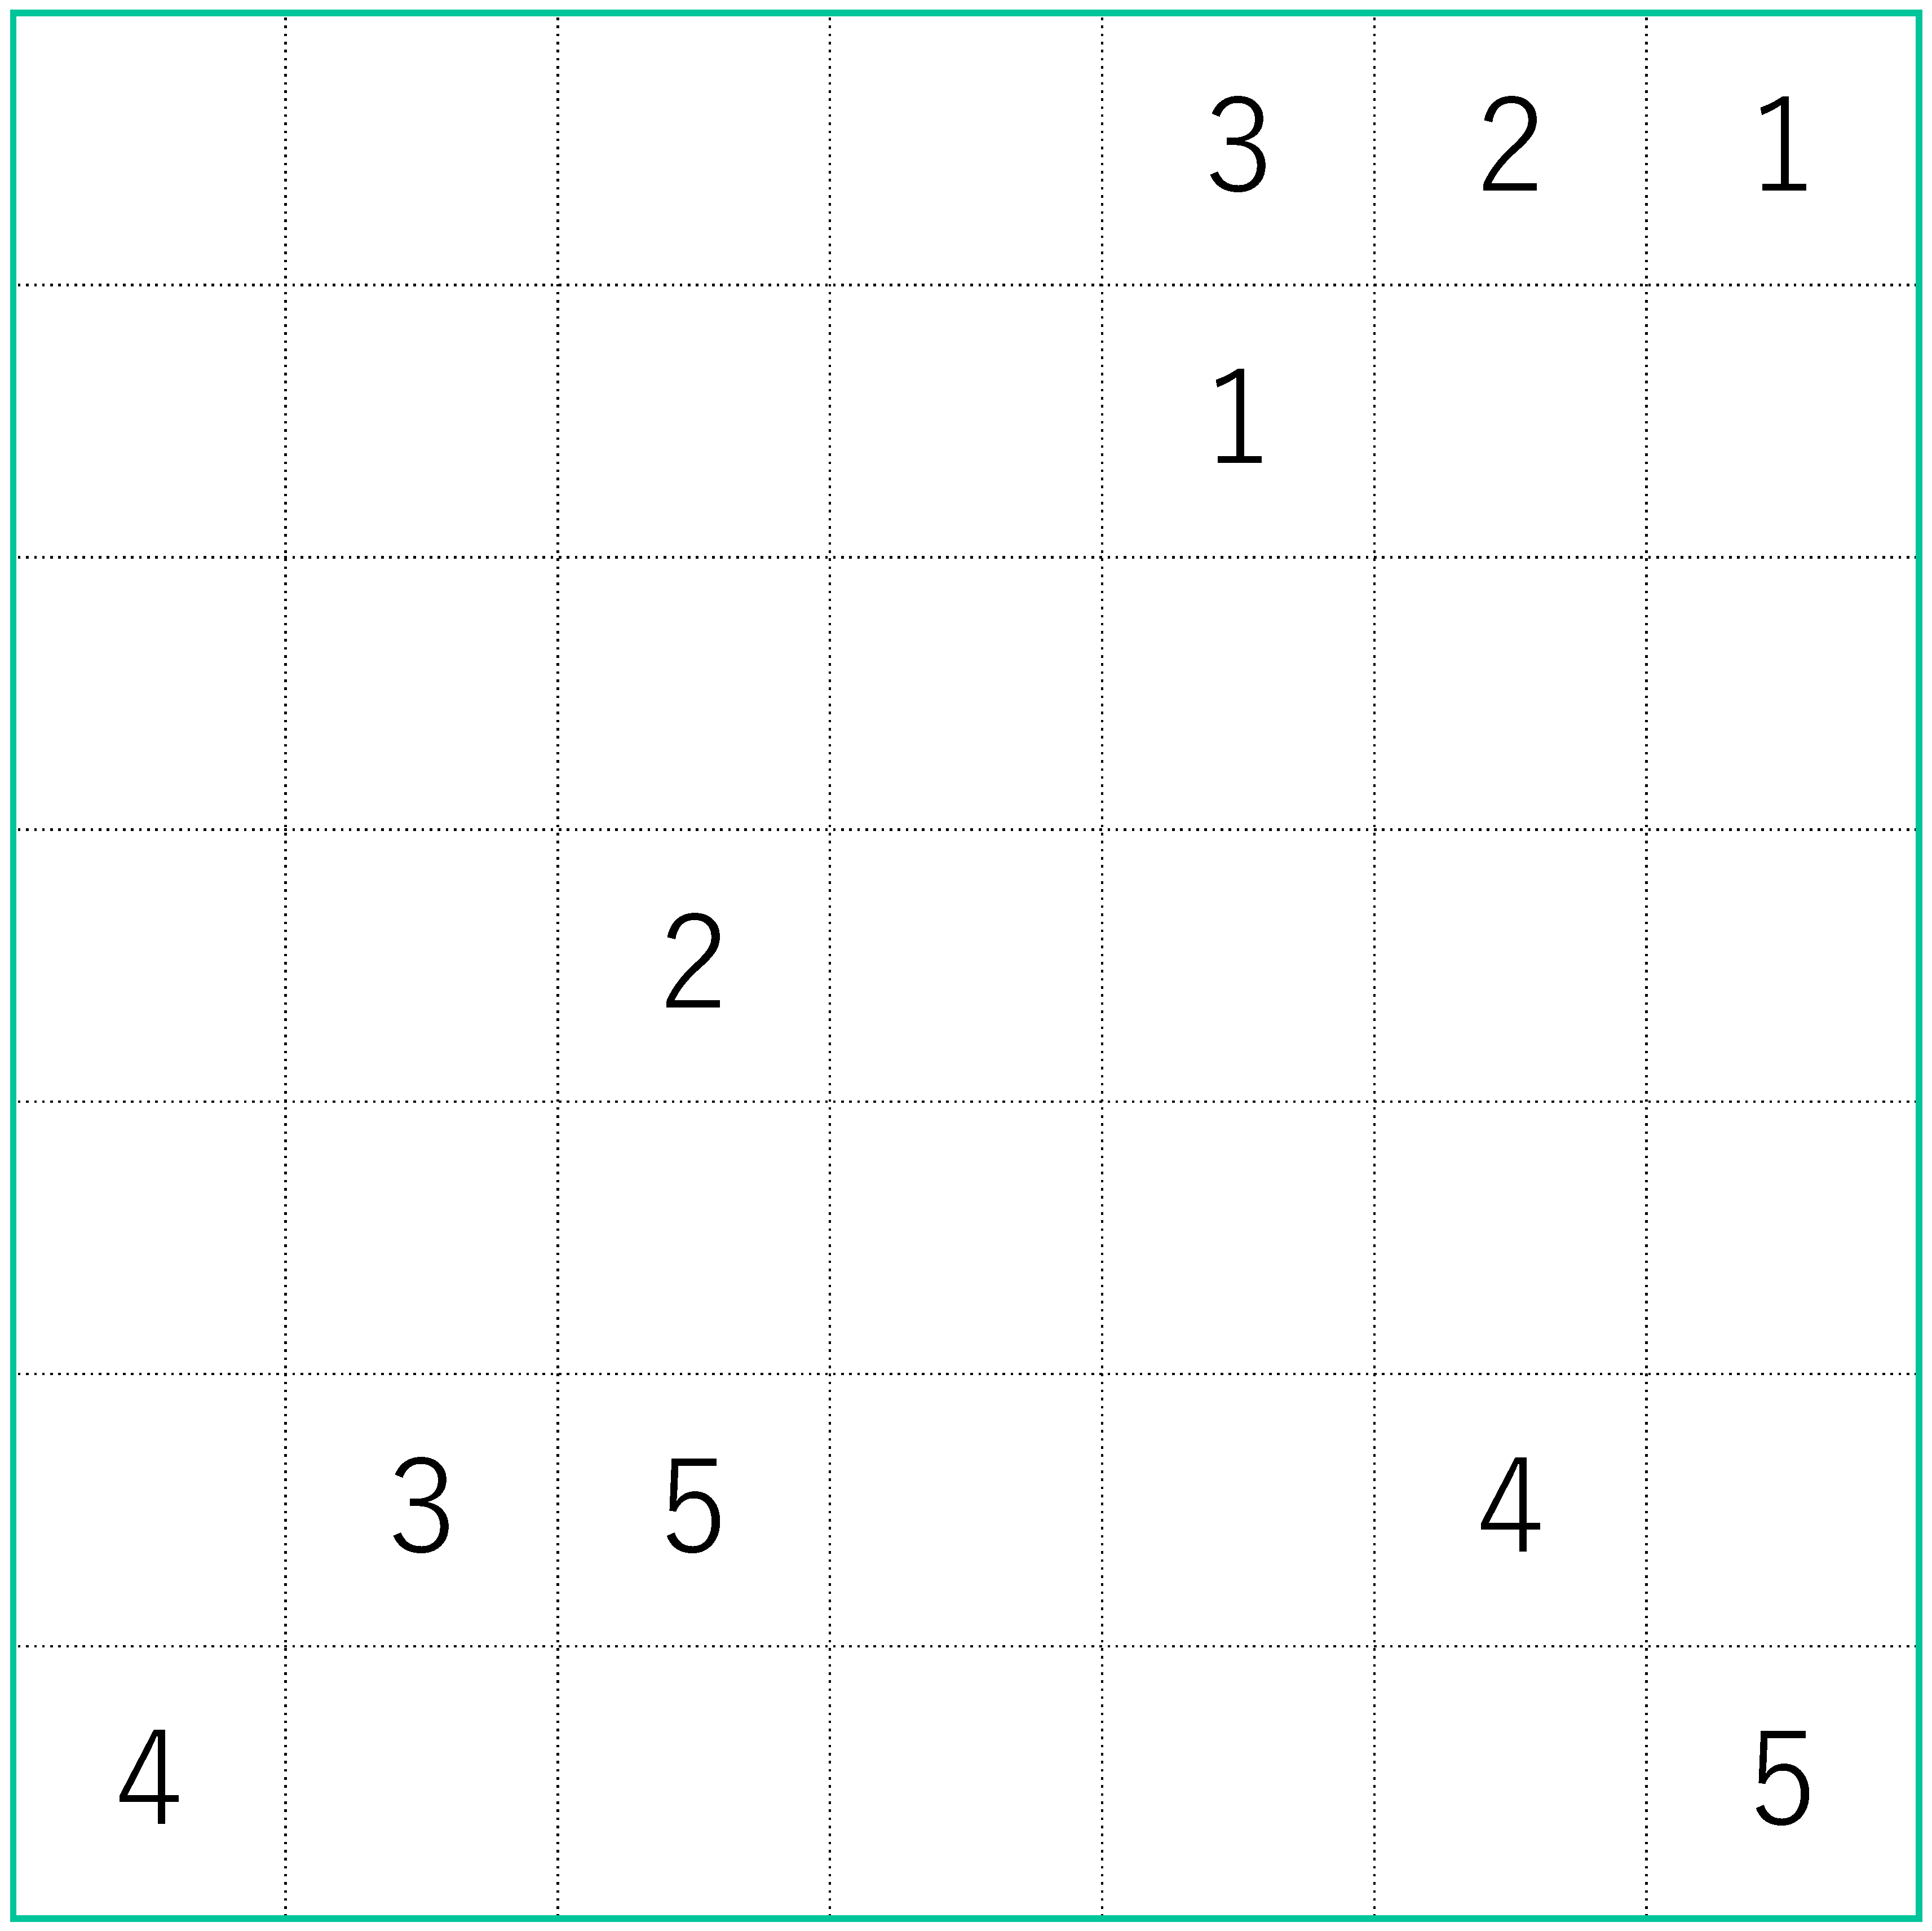
\includegraphics[width=0.85\linewidth,clip]{fig/NumberLinkQuestionReplace.eps}
  \caption{ナンバーリンクの完成盤面(リプレイス後)}
  \label{figure:NumberLinkQuestionReplace}
\end{clearpagefigure}

\begin{clearpagefigure}
  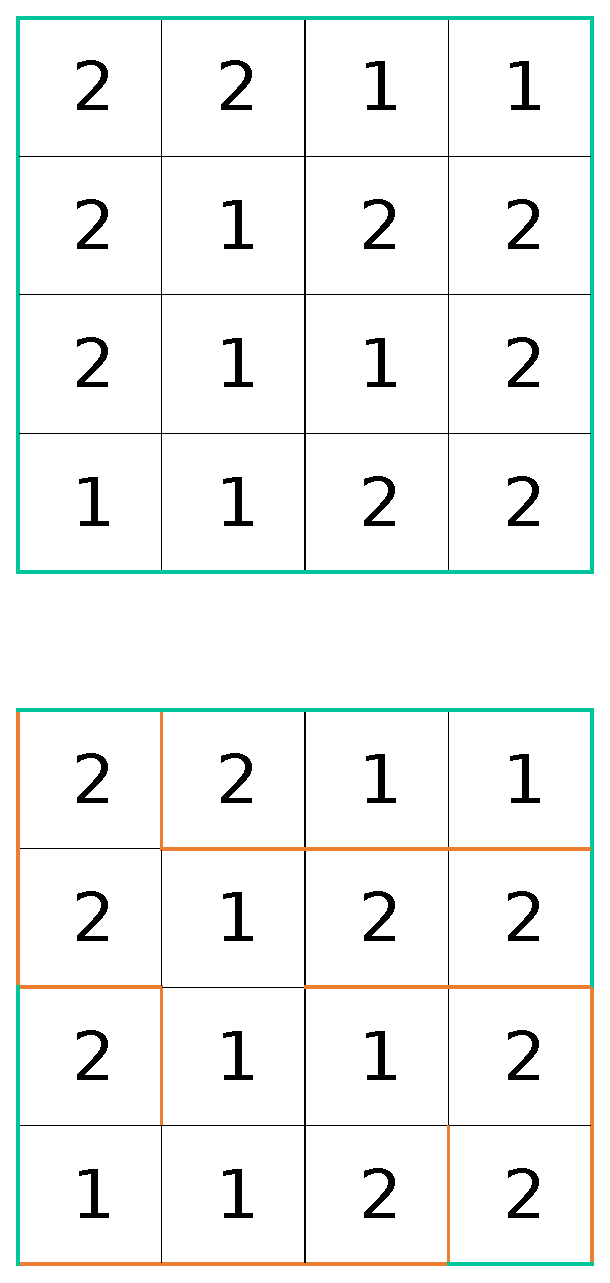
\includegraphics[width=0.5\linewidth,clip]{fig/NewPuzzleRule.eps}
  \caption{新しく作成したパズルルール. 上が非完成盤面, 下が完成盤面. }
  \label{figure:NewPuzzleRule}
\end{clearpagefigure}
